\chapter{Especificación de la API: OpenAPI y \emph{streaming} NDJSON}
\label{cap:AnexoM}

Este anexo documenta la especificación de la API del motor de inteligencia artificial (\emph{AI Engine}), generada automáticamente en formato OpenAPI, y el contrato de \emph{streaming} NDJSON empleado para el resumen en tiempo real. Complementa al Anexo~\ref{cap:AnexoC}, que describe la comunicación entre servicios a alto nivel.

\section{OpenAPI y Swagger UI}

El motor de IA está implementado con FastAPI, que genera automáticamente la especificación \textbf{OpenAPI 3.1} a partir de los modelos de datos (Pydantic) y las firmas de los \emph{endpoints}. La especificación se publica de dos formas:

\begin{itemize}
 \item \textbf{Esquema JSON}: \texttt{GET /openapi.json}, el documento OpenAPI completo, apto para la generación automática de clientes o su importación en herramientas de terceros (Postman, generadores de SDK, etc.).
 \item \textbf{Swagger UI}: \texttt{GET /docs}, interfaz web interactiva para explorar los \emph{endpoints}, consultar los esquemas de petición y respuesta y ejecutar llamadas de prueba directamente desde el navegador (Figura~\ref{fig:swagger}).
\end{itemize}

El backend Phoenix expone análogamente su documentación interactiva en \texttt{GET /docs}, con el esquema OpenAPI en \texttt{GET /api/openapi}.

\begin{figure}[ht]
\centering
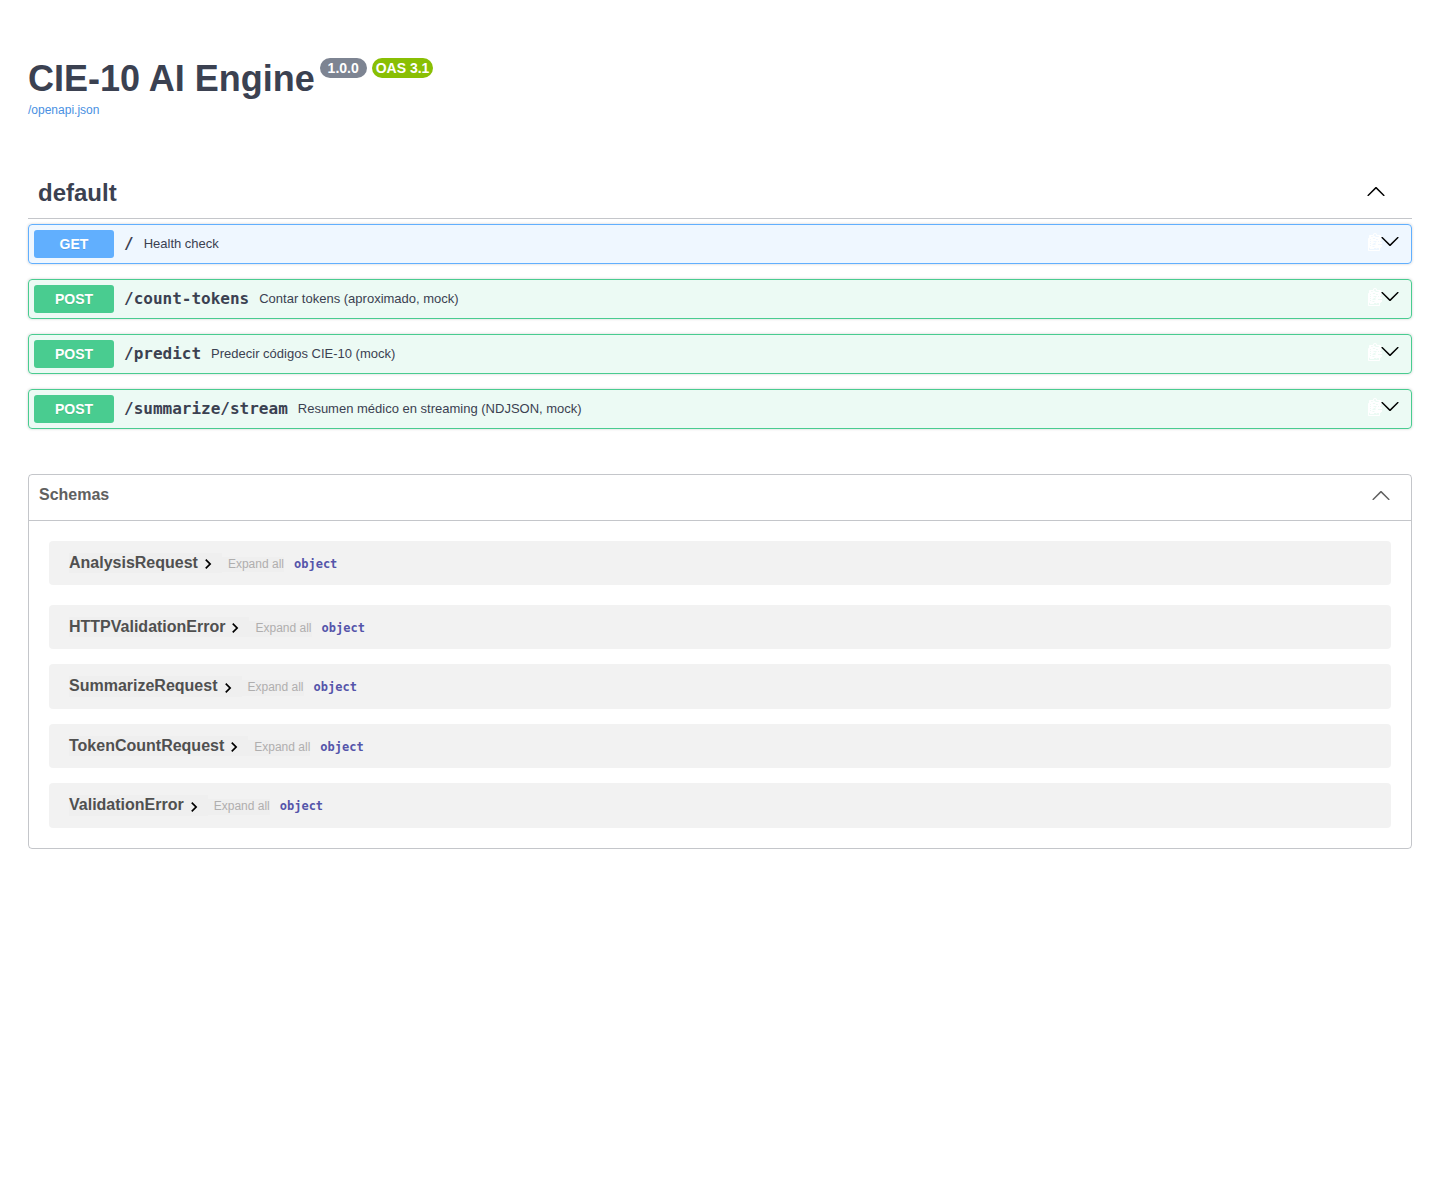
\includegraphics[width=\textwidth]{figs/swagger-ui}
\caption{Swagger UI generada automáticamente por FastAPI para el motor de IA (\texttt{/docs}).}
\label{fig:swagger}
\end{figure}

\paragraph{Obtención en vivo.} Con el sistema en marcha, la especificación completa y siempre actualizada está disponible sin salir del navegador en \texttt{http://localhost:8000/docs} (Swagger UI interactivo) y en \texttt{http://localhost:8000/openapi.json} (esquema OpenAPI 3.1 en JSON, apto para importar en Postman o generar clientes automáticamente). El siguiente fragmento, generado automáticamente por FastAPI, corresponde al \emph{endpoint} \texttt{/predict} y a los esquemas de las dos peticiones que componen un análisis:

{\small
\begin{verbatim}
"/predict": {
 "post": {
 "summary": "Predecir códigos CIE-10",
 "operationId": "predict_codes_predict_post",
 "requestBody": {
 "required": true,
 "content": { "application/json": {
 "schema": { "$ref": "#/components/schemas/AnalysisRequest" } } }
 },
 "responses": {
 "200": { "description": "Successful Response" },
 "422": { "description": "Validation Error", "content": {
 "application/json": { "schema": {
 "$ref": "#/components/schemas/HTTPValidationError" } } } }
 }
 }
}

"AnalysisRequest": {
 "type": "object",
 "required": ["text"],
 "properties": {
 "text": { "type": "string", "title": "Text" },
 "engine": { "type": "string", "title": "Engine", "default": "bert",
 "enum": ["bert", "dict", "both", "fused"] },
 "include_triggers": { "type": "boolean", "title": "Include Triggers",
 "default": false }
 }
}

"ExplainRequest": {
 "type": "object",
 "required": ["text", "codes"],
 "properties": {
 "text": { "type": "string", "title": "Text" },
 "codes": { "type": "array", "items": { "type": "string" },
 "title": "Codes" },
 "method": { "anyOf": [{ "type": "string" }, { "type": "null" }],
 "title": "Method" },
 "top_k": { "type": "integer", "title": "Top K", "default": 5 }
 }
}
\end{verbatim}
}

\section{Endpoints del motor de IA}

La Tabla~\ref{tab:openapi-endpoints} resume los \emph{endpoints} expuestos por el motor de IA.

\begin{table}[h]
\centering
\small
\caption{Endpoints del motor de IA (OpenAPI).}
\label{tab:openapi-endpoints}
\begin{tabular}{llp{7.2cm}}
\hline
\textbf{Método} & \textbf{Ruta} & \textbf{Descripción} \\
\hline
GET & \texttt{/} & Comprobación de estado (\emph{health check}): disponibilidad del servicio y de los modelos. \\
POST & \texttt{/predict} & Predice los códigos CIE-10 de un informe. Parámetro \texttt{engine}: \texttt{bert}, \texttt{dict}, \texttt{both} o \texttt{fused}. \\
POST & \texttt{/explain} & Devuelve los términos que justifican unos códigos ya predichos. \\
POST & \texttt{/count-tokens} & Devuelve el número de \emph{tokens} del texto según el tokenizador del modelo. \\
POST & \texttt{/summarize/stream} & Genera el resumen del informe en \emph{streaming} (NDJSON, token a token). \\
POST & \texttt{/jobs/predict} & Predicción asíncrona: devuelve un \texttt{job\_id} de forma inmediata. \\
POST & \texttt{/jobs/summarize} & Resumen asíncrono: devuelve un \texttt{job\_id} de forma inmediata. \\
GET & \texttt{/jobs/\{job\_id\}} & Consulta el estado y el resultado de un trabajo asíncrono. \\
GET & \texttt{/admin/models} & Lista los modelos publicados y señala cuál está cargado. \\
POST & \texttt{/admin/models} & Carga otro modelo en caliente, sin reiniciar el servicio. \\
POST & \texttt{/admin/summarizer} & Recarga en caliente el modelo de resumen (LLM) y sus \emph{prompts}. \\
GET & \texttt{/metrics} & Métricas en formato Prometheus. \\
\hline
\end{tabular}
\end{table}

\section{Esquemas de petición y respuesta}

\subsection{POST /predict}

Petición:

{\small
\begin{verbatim}
{
 "text": "<informe clínico en español>",
 "engine": "bert" // opcional: "bert" (def.), "dict", "both" o "fused"
}
\end{verbatim}
}

Respuesta: un objeto con el campo \texttt{cards}, que contiene una única tarjeta de tipo \texttt{codes} (el resumen se solicita por separado con \texttt{/summarize/stream}):

{\small
\begin{verbatim}
{
 "cards": [
 {
 "type": "codes",
 "content": [
 {
 "code": "E11.9",
 "description": "Diabetes mellitus tipo 2 sin complicaciones",
 "reason": "Capítulo IV: confianza 91.0%",
 "confidence": 0.91,
 "relative_confidence": 0.86,
 "triggers": ["diabetes", "glucosa"],
 "engine": "bert"
 }
 ]
 }
 ]
}
\end{verbatim}
}

El campo \texttt{confidence} es la probabilidad bruta de la sigmoide; \texttt{relative\_confidence} es su normalización \emph{min-max} dentro del conjunto devuelto (véase la sección~\ref{sec:confianza-predicciones}); \texttt{triggers} son los términos del informe que motivan la predicción (véase la sección~\ref{sec:explicabilidad}); y \texttt{engine} identifica el motor de origen.

\subsection{POST /explain}

La atribución de importancia viaja en un \emph{endpoint} separado porque cuesta del orden de cien veces más que predecir: mide el efecto real de eliminar cada palabra del informe, lo que exige una pasada del \emph{encoder} por palabra. Atarla a \texttt{/predict} obligaba al usuario a esperar por una información que todavía no estaba consultando, ya que primero lee la lista de códigos y solo después despliega uno para saber por qué se ha propuesto. Separadas, los códigos se devuelven en cuanto están y las palabras llegan después.

Por ese motivo \texttt{/predict} admite el campo \texttt{include\_triggers}, desactivado por defecto: activarlo reproduce el comportamiento anterior, en el que la respuesta completa esperaba a la atribución.

La petición indica el texto, los códigos que se quieren justificar y, opcionalmente, la estrategia. La respuesta incluye siempre el método empleado, de modo que ante un término inesperado se puede saber si lo produjo la versión fiel o una de las rápidas (Tabla~\ref{tab:explain-metodos}).

\begin{table}[h]
\centering
\small
\caption{Estrategias de atribución admitidas por \texttt{/explain}.}
\label{tab:explain-metodos}
\begin{tabular}{p{3.3cm}p{9.5cm}}
\hline
\textbf{Método} & \textbf{Descripción} \\
\hline
\texttt{diccionario} & No emplea el \emph{encoder}: devuelve las frases clínicas que hicieron coincidencia por expresión regular. Responde en centésimas de segundo. En el motor fusionado estos términos ya viajan con la predicción sin coste adicional, de modo que esta vía sirve al motor neuronal, que no ejecuta el diccionario. \\
\texttt{gradiente\_filtrado} & Una pasada hacia atrás ordena las palabras candidatas y solo se enmascaran las más prometedoras. \\
\texttt{exhaustivo} & Pregunta por todas las palabras. Es la referencia fiel y la más costosa. \\
\texttt{divide\_y\_venceras} & Enmascara grupos y descarta el que no altera ningún \emph{logit}. Documentado como resultado negativo: en este corpus resulta más lento que el exhaustivo. \\
\hline
\end{tabular}
\end{table}

Los cuatro motores no son variantes del mismo cálculo. \texttt{bert} y \texttt{dict} devuelven las predicciones de un solo clasificador; \texttt{both} devuelve las de ambos concatenadas, cada código con su motor de origen, y deja la reconciliación al cliente; \texttt{fused} combina las puntuaciones de los dos \emph{antes} de ordenar, sumando al \emph{logit} de cada código una bonificación proporcional a la confianza con que el diccionario ha detectado su bloque (Anexo~\ref{cap:AnexoF}, sección~\ref{sec:anexoF-fusion}). Este último emplea un umbral propio, expresado en el espacio de la puntuación combinada, y añade a cada código los campos \texttt{score\_model} y \texttt{score\_dict} con la contribución literal de cada fuente, además de \texttt{dict\_support} y \texttt{trigger\_detail}, que etiqueta cada término explicativo con su procedencia.

\subsection{GET / y POST /count-tokens}

{\small
\begin{verbatim}
GET / -> {"status": "online", "model_loaded": true,
 "dict_loaded": true, "summarizer_loaded": true, ...}

POST /count-tokens {"text": "..."} -> {"token_count": 349}
\end{verbatim}
}

\section{Streaming NDJSON: \texttt{POST /summarize/stream}}

El resumen del informe se entrega mediante \textbf{NDJSON} (\emph{newline-delimited JSON}): la respuesta es un flujo en el que \textbf{cada línea es un objeto JSON independiente}, lo que permite al cliente renderizar el texto de forma incremental (efecto \emph{typewriter}) sin esperar a que el LLM termine. El tipo de contenido de la respuesta es \texttt{application/x-ndjson}.

El protocolo es el siguiente: se emite una línea por cada fragmento generado y una línea final que señala el fin del flujo; ante un error se emite una línea de error antes de cerrar.

{\small
\begin{verbatim}
{"token": "Paciente "}
{"token": "de 70 "}
{"token": "años con "}
...
{"done": true}
\end{verbatim}
}

En caso de fallo del generador, la última línea es \texttt{\{"error": "<mensaje>"\}} en lugar de \texttt{\{"done": true\}}. Si el modelo de resumen no está cargado, el servicio devuelve un único fragmento con un resumen estadístico de reserva y a continuación \texttt{\{"done": true\}}, de modo que el cliente siempre recibe una respuesta bien formada.

El backend retransmite cada línea recibida al frontend a través del canal WebSocket como eventos \texttt{summary\_token} (véase el Anexo~\ref{cap:AnexoC}), desacoplando así el protocolo interno (NDJSON) del protocolo con el cliente (WebSocket).
